\section{Øving 8}
\subsection{Selvangivelse}

\begin{center}
\begin{tabular}{ |c|c|c|}
\hline
Oppgave & Status & Kommentar \\
\hline
1 & OK & Fungerer som den skal \\ 
\hline
2 & OK & Fungerer med hele steps men halfstep er standard. \\  
\hline
3 & OK & Regulator fungerer som den skal \\
\hline
4 & OK & Fungerer som den skal \\
\hline
5 & 90\% & Trege syklustider gir tidvis uventede  \\
& & resultater under for eksempel kalibrering. \\
\hline
6 & OK & Half-stepping er implementert. \\
\hline
7 & OK & Besvart i denne oppgaven \\
\hline
\end{tabular}
\label{tab:Parameters}
\end{center}

\subsection{Oppgave 1}
\textbf{\textit{ Simulator og visualisering: }}
\newline
I oppgaven skulle man ha tilsvarende inn- og utganger som funksjonsblokken til venstre. Funksjonsblokken til høyre i \ref{fig:Simulator}, viser hvordan programmets simuleringsblokk egentlig ser ut. Eneste forskjellen er at den gir ut en vinkel slik at vingen i visualiseringen vet hvilken vinkel den skal stille seg inn på.

\begin{figure}[h!]
    \centering
    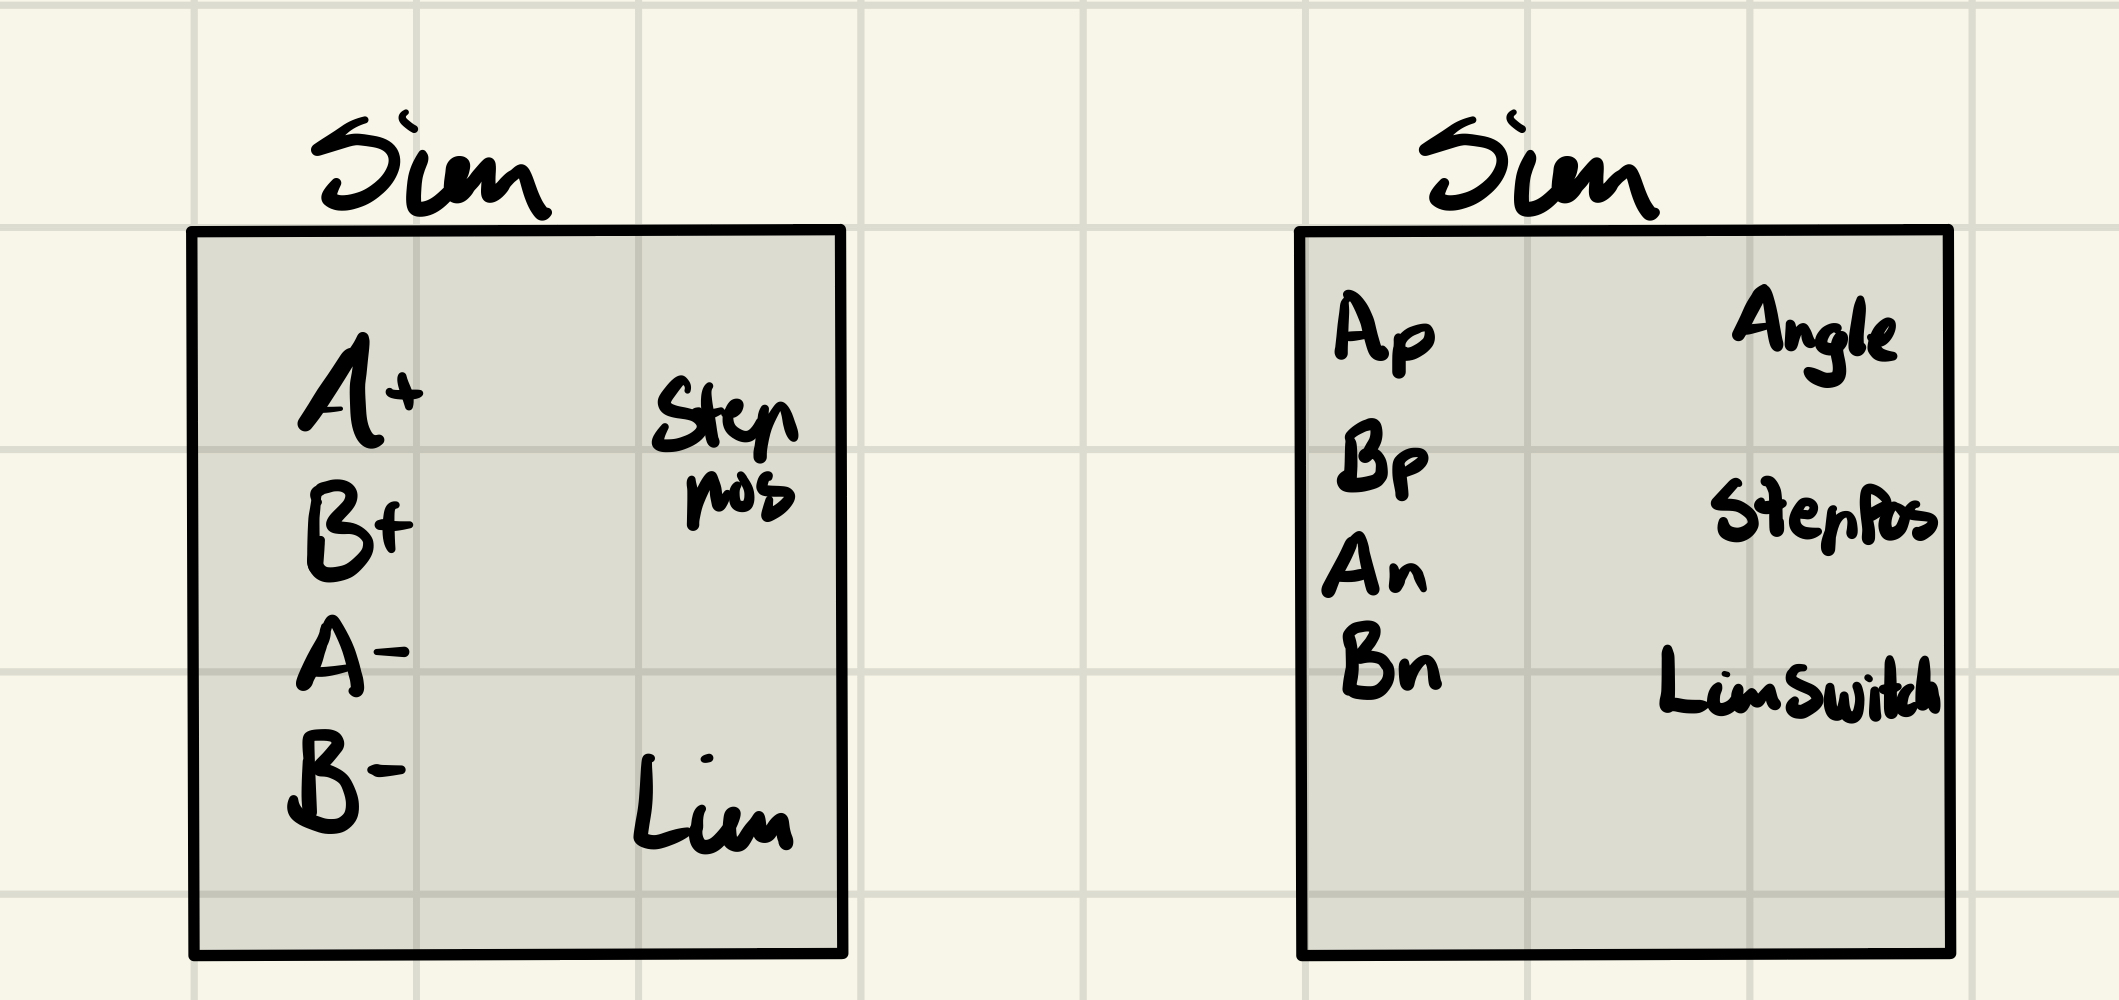
\includegraphics[width = 0.5\textwidth]{Images/Simulator.jpeg}
    \caption{Tegning av simulator funksjons blokken.}
    \label{fig:Simulator}
\end{figure}

\begin{figure}[h!]
    \centering
    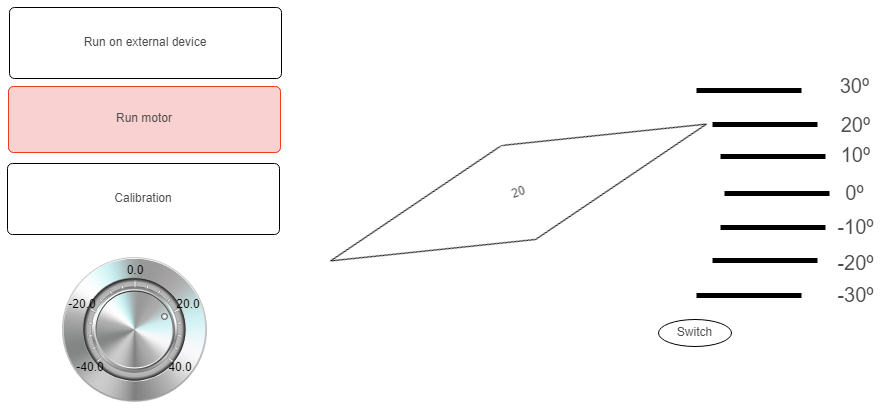
\includegraphics[width = 0.5\textwidth]{Images/Visu.png}
    \caption{Visualisering til programmet.}
    \label{fig:Driver}
\end{figure}

\subsection{Oppgave 2}
\textbf{\textit{Step driver:}}
\newline
Step driveren skal ha inn- og utganger tilsvarende venstre side i figur \ref{fig:Driver}. Den faktisk benyttede funksjonsblokken er til høyre i bildet. Forskjellen er input variabelen StepDelay som kan brukes til å styre hastigheten på steppermotoren. Alternativt kan man styre hastigheten med syklustiden på PLS og gi  StepDelay verdien 0.

\begin{figure}[h!]
    \centering
    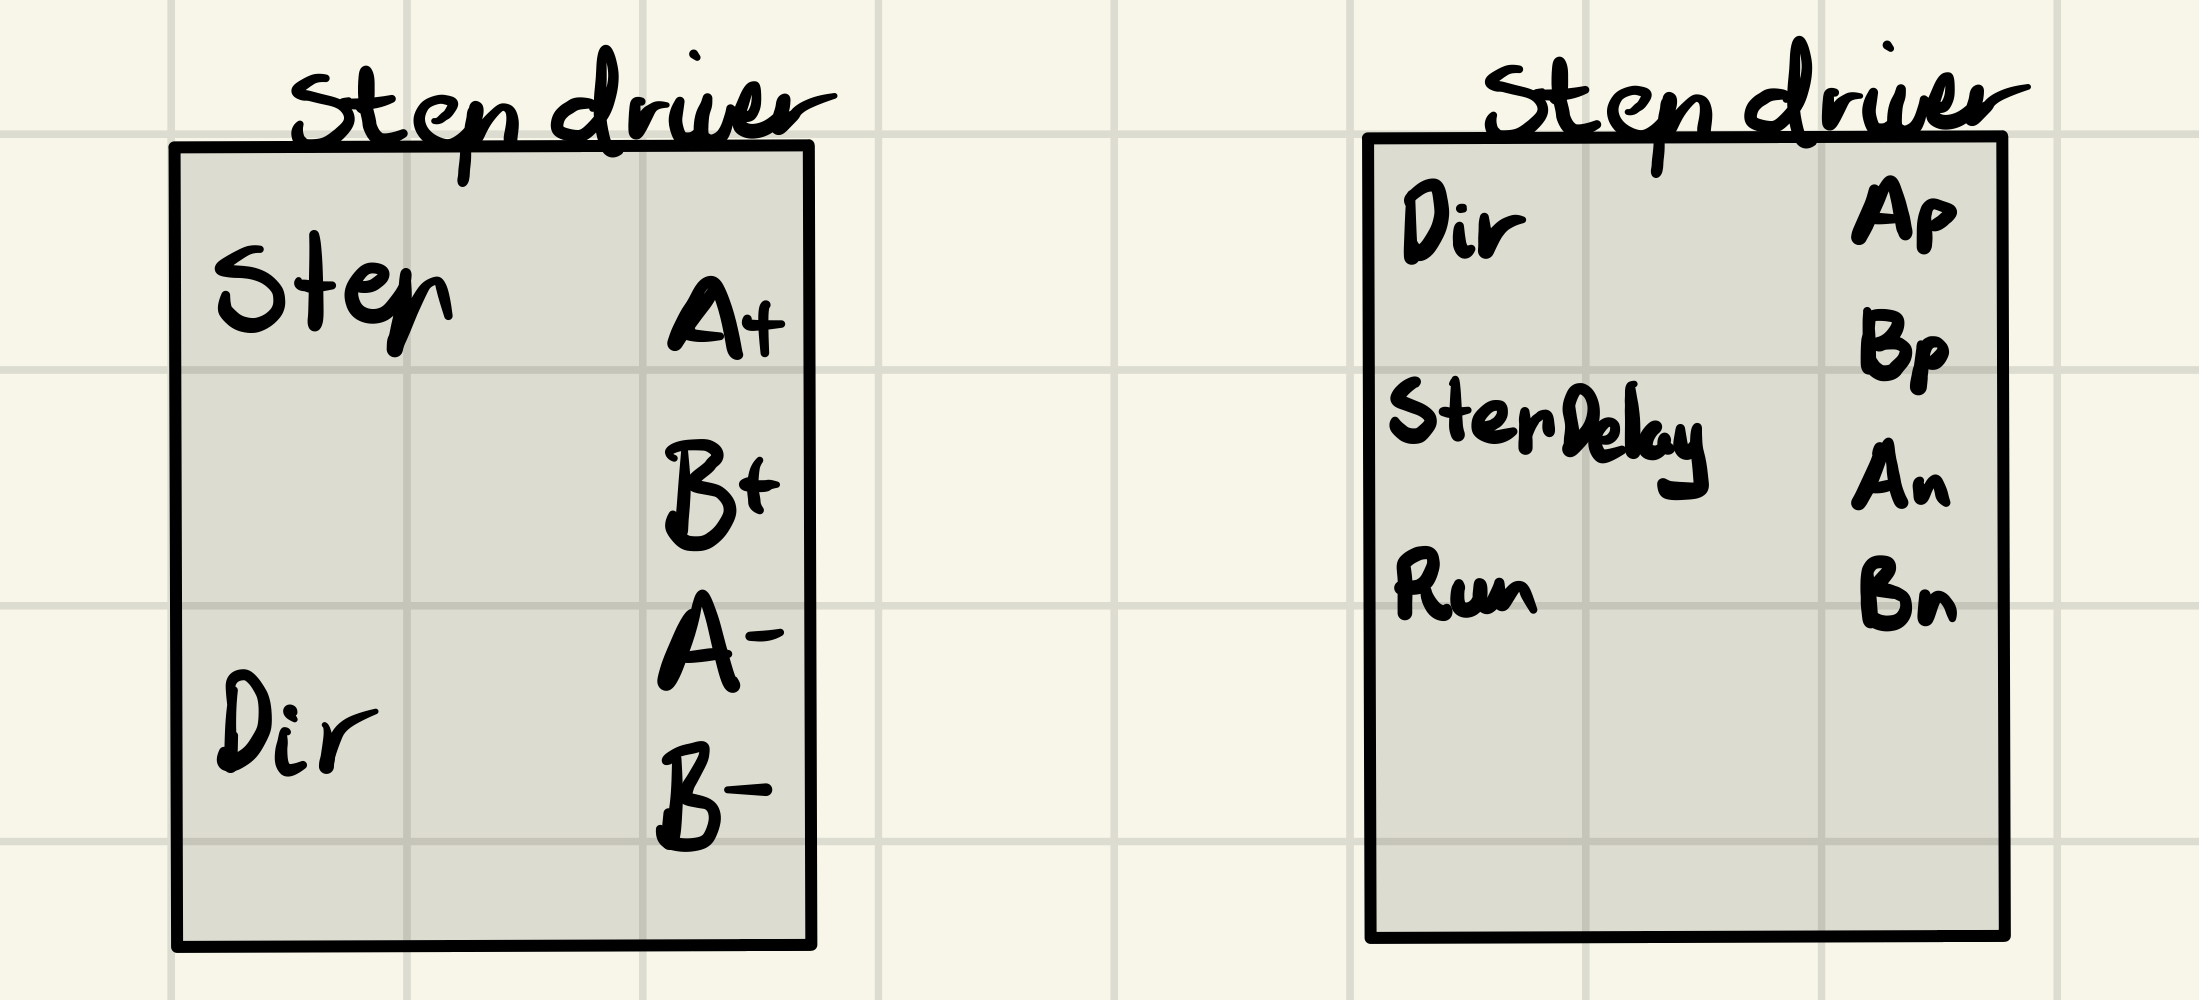
\includegraphics[width = 0.5\textwidth]{Images/Driver.jpeg}
    \caption{Tegning av stepper-driver funksjons blokken.}
    \label{fig:Driver}
\end{figure}

\subsection{Oppgave 3}
\textbf{\textit{Regulator:}}
\newline
I oppgave 3 skal man lage regulatoren til systemet. Den skulle ha inn og utganger tilsvarende figuren til venstre i figur \ref{fig:Regulator}. Den faktiske funksjonsblokken til regulatoren hadde tilsvarende inn- og utganger som funksjonen til høyre.

\begin{figure}[h!]
    \centering
    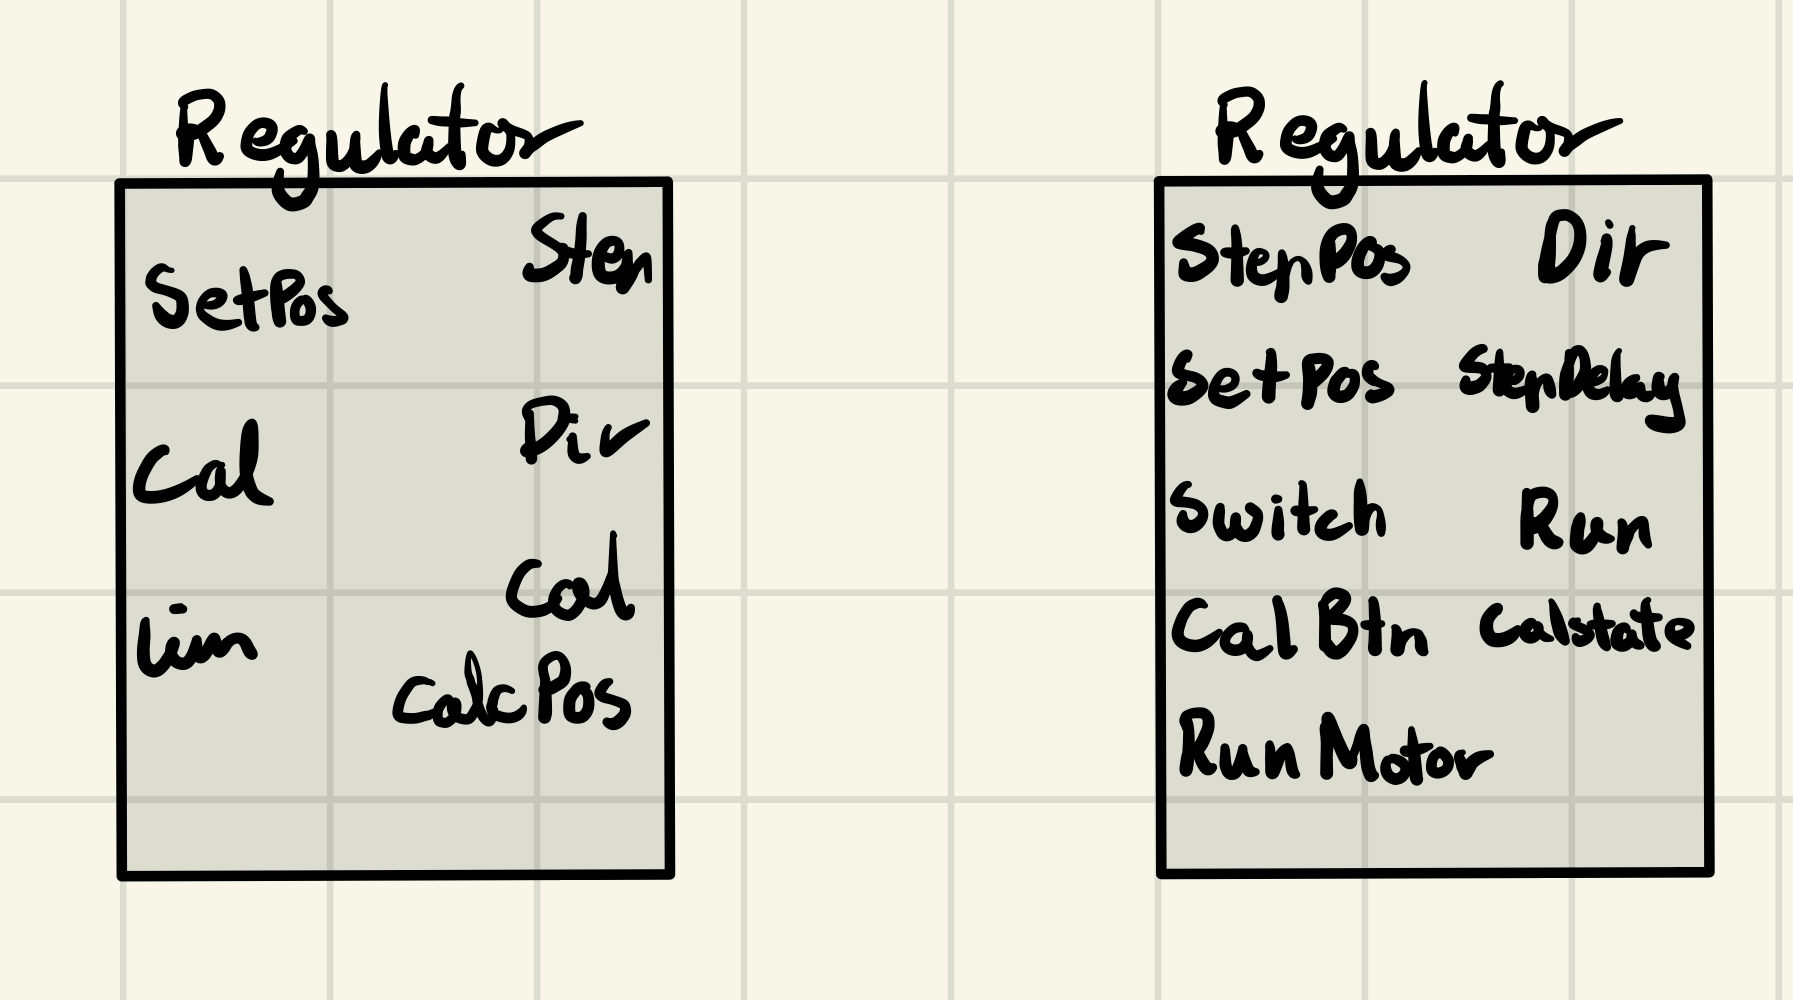
\includegraphics[width = 0.5\textwidth]{Images/Regulator.jpeg}
    \caption{Tegning av regulator funksjons blokken.}
    \label{fig:Regulator}
\end{figure}

\subsection{Oppgave 4}
\textbf{\textit{Fysisk modell:}}
\newline
Oppgaven går ut på å lage en knapp for visualisering med fysisk modell og visualisering. Dette fungerte da jeg koblet opp modellen. 

\subsection{Oppgave 5}
\textbf{\textit{Digital tvilling:}}
\newline
Da jeg koblet opp systemet så fungerte logikken i systemet i sin helhet, men det oppførte seg ikke helt som forventet. Da simulatoren og den fysiske modellen skulle kjøre sammen så gikk simulatoren veldig mye fortere enn den fysiske modellen. Kalibreringen fungerte men for den simulerte modellen så kom den da ikke på forventet plass når den følger den fysiske modellen.

Da databladet ble undersøkt ble det avdekket at step size på motoren til den fysiske modellen er $\frac{360 \degree}{1024}$ hvis man bruker hele steps \cite{Stepper-motor-datasheet}. Det tilsvarer en step size på 0.3515 \degree. Step size på stepper motoren er liten fordi den har et innebygd 1:32 gir. Hvis man half-stepper kan man oppnå en steg størrelse på 0.1758 \degree.

Løsningen ble å sette posisjonen til visualiseringen til - 40 grader, altså step posisjon 0, etter motoren er kalibrert. Ved å gjøre dette kan man få lik oppførsel på det virkelige systemet og det virituelle.

\subsection{Oppgave 6 - Half-Step}
\textbf{\textit{Half-stepping:}}
\newline
\begin{center}
\begin{tabular}{ |c|c|c|c|c|}
\hline
Tilstand & Channel 1 & Channel 3 & Channel 2 & Channel 4 \\
 & A+ & B+ & A- & B - \\
\hline
0 & 1 & 0 & 0 & 0 \\ 
\hline
1 & 1 & 1 & 0 & 0 \\ 
\hline
2 & 0 & 1 & 0 & 0 \\ 
\hline
3 & 0 & 1 & 1 & 0 \\ 
\hline
4 & 0 & 0 & 1 & 0 \\ 
\hline
5 & 0 & 0 & 1 & 1 \\ 
\hline
6 & 0 & 0 & 0 & 1 \\ 
\hline
7 & 1 & 0 & 0 & 1 \\ 
 \hline
\end{tabular}
\label{tab:Halfstep}
\end{center}

Oppgaven gikk ganske greit. Løsningen ble å lage en egen driver og simulator for half stepping. Driveren har states tilsvarende tabell \ref{tab:Halfstep}. Simulatoren for half-stepping inkrementerer med kun et halvt steg for hver tilstandsendring slik at man kan simulere steget mellom to spoler.

\subsection{Oppgave 7}
\textbf{\textit{Lærdom av oppgaven:}}
\newline
Denne oppgaven har gitt meg godt læringsutbytte. Vanskelighetsgraden var i mine øyne svært passende. Oppgaven lærte meg mer om verdien av en digital tvilling for å teste systemer. Det lærte meg også om funksjonen til en stepper motor og hvor forskjellig hver motor kan være hver for seg. Jeg ble overrasket over hvor rask syklustid PLS og steppermotoren håndterte under steppingen. Jeg opplevde dette som en kul oppgave. Eneste frustrasjonen jeg har er software vi bruker som jeg opplever som kronglete, treigt og ustabilt.